\mode*

% Since this a solution template for a generic talk, very little can
% be said about how it should be structured. However, the talk length
% of between 15min and 45min and the theme suggest that you stick to
% the following rules:  

% - Exactly two or three sections (other than the summary).
% - At *most* three subsections per section.
% - Talk about 30s to 2min per frame. So there should be between about
%   15 and 30 frames, all told.


\section{Flernivåsäkerhet}

\subsection{Bell--LaPadula säkerhetspolicymodell}
\begin{frame}{\insertsubsectionhead}
  \begin{description}
    \item[Säkerhetspolicymodell] Uttrycker koncist skyddegenskaperna ett system 
      måste ha.
      Ligger till grund för formell analys.
    \item[Säkerhetsmål] Mer detaljerad beskrivning av given implementation av 
      mekanismer, hur dessa relaterar till mål (härledda från policymodellen).
      Grund för testning och utvärdering.
    \item[Skyddsprofil] En implementationsoberoende version av säkerhetsmålet, 
      används för att jämföra olika system.
    \item[Säkerhetspolicy] Ett dokument som tydligt uttrycker målen våra 
      säkerhetsmekanismer ska uppnå.
      Används ofta som synonym till både säkerhetspolicymodell och 
      säkerhetsmål.
  \end{description}
\end{frame}
\begin{frame}{\insertsubsectionhead}
  \begin{itemize}
    \item Ett säkert system bör göra en eller två saker väl -- det måste vara 
      enkelt.
    \item Dessa saker ska säkras av lika enkla mekanismer -- som då går att 
      analysera.
    \item Dessa mekanismer utgör vad som kallas \emph{trusted computing base 
      (TCB)}.
    \item Bell--LaPadula är exempel på en sådan säkerhetspolicymodell.
    \item Utvecklades av Bell och LaPadula under 1970-talet.
    \item Syftet är att skydda fleranvändarsystem.
  \end{itemize}
\end{frame}
\begin{frame}{\insertsubsectionhead}
  \begin{itemize}
    \item Andra världskriget och Kalla kriget ledde NATO-länderna att utveckla 
      en gemensam klassificeringsmodell för känsliga dokument.
    \item Klassificeringarna utgör etiketter som är ordnade i nivåer; från 
      \emph{ej sekretessbelagd (Unclassified)} till \emph{förtrolig 
      (Confidential)}, \emph{hemlig (Secret)} och \emph{kvalificerat hemlig 
      (Top Secret)}.
    % XXX add reference for labels of classification
    \item EU har även \emph{begränsad (Restricted)}.
    \item En individ har \emph{behörighet (clearance)} för en säkerhetsnivå.
  \end{itemize}
\end{frame}
\begin{frame}{\insertsubsectionhead}
  \begin{itemize}
    \item En individ kan läsa information som är klassificerat till alla nivåer 
      upp till den nivå denne är behörig.
    \item Det krävs speciella personer för att avklassificera dokument.
    \item Till de olika nivåerna hör olika skyddsnivåer.
  \end{itemize}
\end{frame}
\begin{frame}{\insertsubsectionhead}
  \begin{itemize}
    \item Vi kan även lägga till speciella kodord till klassificeringarna.
    \item En klassificering med ett eller flera kodord utgör en 
      \emph{säkerhetskategori (security category eller compartment)}.
    \item Detta ger multilateral säkerhet.
  \end{itemize}
\end{frame}
\begin{frame}{\insertsubsectionhead}
  \begin{block}{Bell--LaPadulamodellen (BLP)}
    \begin{description}
      \item[NRU] (Simple security property, No read up) Ingen process får läsa 
        data från en högre nivå.
      \item[NWD] (*-property, No write down) Ingen process får skriva data till 
        en lägre nivå.
    \end{description}
  \end{block}
  \begin{itemize}
    \item Bell och LaPadulas säkerhetsmodell publicerades 1973.
    \item System som implementerar den kallas oftast \emph{flernivåsäkra system 
      (multilevel secure, MLS)}.
    \item Information kan inte flöda nedåt, bara uppåt.
    \item System som implementerar denna typ av policy oberoende av användaren 
      sägs ha \emph{obligatorisk åtkomstkontroll (mandatory access control)}.
  \end{itemize}
\end{frame}
\begin{frame}{\insertsubsectionhead}
  \begin{block}{Utökning av BLP}
    Inför \emph{tranquility property}, finns två varianter:
    \begin{description}
      \item[Stark] Säkerhetsklassificeringar förändras aldrig under systemets 
        gång.
      \item[Svag] Säkerhetsklassificeringar förändras aldrig så att 
        säkerhetspolicyn bryts.
    \end{description}
  \end{block}
  \begin{itemize}
    \item Anledningen till den svaga är \emph{principle of least privilege}.
    \item Börja på lägsta säkerhetsnivån och öka allteftersom data med högre 
      nivå används -- \emph{high watermark principle}.
    \item Vad händer då här en ny fil skapas senare?
    \item Det kommer att behövas en \emph{trusted subject} för av 
      avklassificera.
  \end{itemize}
\end{frame}

\subsection{Bibamodellen}
\begin{frame}{\insertsubsectionhead}
%  \begin{block}{Bibamodellen}
%  \end{block}
  \begin{itemize}
    \item Vanligen kallad ''Bell--LaPadula upp-och-ned''.
    \item Används för integritet medan BLP används för konfidentialitet.
    \item Kan läsa data från högre nivåer men inte skriva till dem.
    \item Följaktligen används \emph{low watermark principle}.
    \item Lägre nivåer innehåller osäkra data och data baserat på dessa kan 
      därför inte vara mindre osäkra.
    \item LOMAC i Linux där en process nedgraderades från hög till låg då den 
      mottog data från nätverket.
    \item Windows införde därefter liknande system för att säkra bland annat 
      Internet Explorer.
  \end{itemize}
\end{frame}

\subsection{Alternativa modeller}
\begin{frame}{\insertsubsectionhead}
  \begin{itemize}
    \item \emph{Noninterference} kom 1982.
    \item Saker som händer på hög säkerhetsnivå har ingen effekt på vad låg 
      säkerhetsnivå kan se.
    \item \emph{Nondeducability} kom 1986.
    \item Förenkling av tidigare: bevisa att låg nivå inte kan härleda med 
      \SI{100}{\%} säkerhet vad som händer på hög.
    \item Även om det går att se är det oförståeligt.
    \item Ett exempel på tillämpningsområde är ett nätverk med datorer med både 
      hög och låg säkerhetsklassning.
  \end{itemize}
\end{frame}
\begin{frame}{\insertsubsectionhead}
  \begin{itemize}
    \item \emph{Type enforcement (TE)} tilldelar \emph{domäner} för subjekt och 
      \emph{typer} för objekt.
    \item Därefter skapas en matris som specificerar tillåtna domän--domän- 
      respektive domän--typ-kombinationer.
    \item Utökades till \emph{Domain and Type Enforcement (DTE)}.
    \item Ger ett komplext språk att specificera policyer.
  \end{itemize}
\end{frame}
\begin{frame}{\insertsubsectionhead}
  \begin{itemize}
    \item Rollbaserad åtkomstkontroll (\emph{role-based access control, RBAC}) 
      har sitt ursprung i bankvärlden.
    \item Baseras på användarens funktion som den utför snarare än en given 
      användare.
    \item Det är skillnad på ''Daniel läraren'' och ''Daniel studenten''.
    \item Men inte skillnad på ''Daniel läraren'' och ''Lennart läraren''.
    \item Mina rättigheter kan således begränsas beroende på vad jag gör: inte 
      installera program när jag läser e-post -- och alltså skydda mot 
      sabotageprogram.
    \item Kan då hantera både konfidentialitet och integritet.
    \item Detta implementeras i Linux genom TE och DTE.
  \end{itemize}
\end{frame}
\begin{frame}{\insertsubsectionhead}
  \begin{itemize}
    \item Virtualisering är ett sätt att implementera olika nivåer och separera 
      dem.
    \item NSA implementerade NetTop: en modifierad version av VMware.
    \item Linux som bassystem med Windows som virtuella maskiner.
    \item Anställda fick datorer som såg ut som Windows.
    \item Säkerhetsfolket fick hög säkerhet med separerade säkerhetsnivåer.
    \item Finns dock problem:
      Hur vet du vilken virtuell maskin som mikrofonen är ansluten till, hemlig 
      nivå eller ej sekretessbelagd?
  \end{itemize}
\end{frame}

\subsection{Hemliga kanaler}
\begin{frame}{\insertsubsectionhead}
  Vad händer om jag skriver till en fil som redan finns på högre 
  konfidentialitetsnivå?
\end{frame}
\begin{frame}{\insertsubsectionhead}{NRL-pump}
  \begin{itemize}
    \item Används för att begränsa bandbredden för hemliga kanaler.
  \end{itemize}
\end{frame}
\begin{frame}{\insertsubsectionhead}{Logistiksystem}
  \begin{itemize}
    \item Ett militärlager med hemlig utrustning.
    \item En logistiker som inte har behörighet för hemlig, vad ska denne se?
  \end{itemize}
\end{frame}


\section{Multilateral säkerhet}
\begin{frame}{\insertsubsectionhead}
  \begin{quote}
    Privacy is a transient notion.
    It started when people stopped believing that God could see everything and 
    stopped when governments realised there was a vacancy to be filled.
  \end{quote}
  \begin{flushright}
    Roger Needham
  \end{flushright}
\end{frame}

\subsection{Gittermodellen (lattice model)}
\begin{frame}{\insertsubsectionhead}
  \begin{figure}
    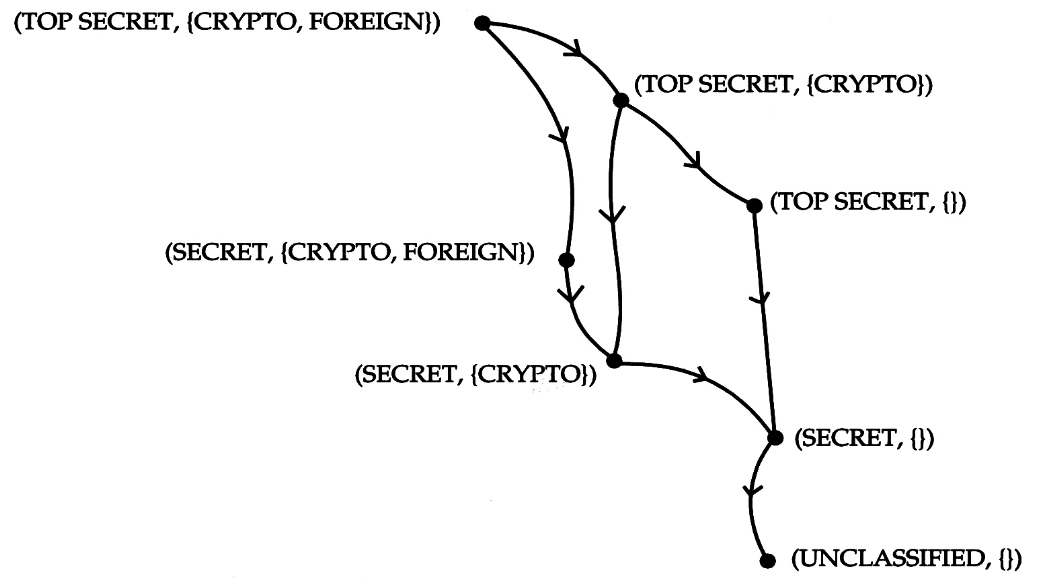
\includegraphics[height=0.7\textheight]{lattice.png}
    \caption{Exempel på gittermodellen, idén är att BLP bara behöver en 
    partiell ordning.}
  \end{figure}
\end{frame}

\subsection{Kinesiska muren-modellen}
\begin{frame}{\insertsubsectionhead}
  \begin{itemize}
    \item Utvecklades av Brewer och Nash.
    \item Har sitt ursprung hos bankerna.
    \item \emph{Separation of duty}: en användare får utföra \(A\) eller \(B\), 
      men inte båda.
    \item En systemadministratör får göra allt i ett system, men loggarna finns 
      hos någon annan systemadministratör.
  \end{itemize}
\end{frame}
\begin{frame}{\insertsubsectionhead}
  \begin{block}{Kinesiska muren}
    Låt \(c\) beteckna en resurs, \(y(c)\) är \(c\):s ägare och \(x(c)\) är 
    dess intressekonfliktklass.
    Då kan Kinesiska muren uttryckas enligt BLP som följande:
    \begin{description}
      \item[Simple security property] Ett subjekt \(s\) har tillgång till \(c\) 
        om och endast om för alla \(c^\prime\) som \(s\) kan \emph{läsa från} 
        gäller \(y(c)\notin x(c^\prime)\) eller \(y(c) = y(c^\prime)\).
      \item[*-property] Ett subjekt \(s\) kan skriva till \(c\) om och endast 
        om \(s\) inte kan läsa något \(c^\prime\) sådant att \(x(c^\prime)\neq 
        \emptyset\) och \(y(c)\neq y(c^\prime)\).
    \end{description}
  \end{block}
\end{frame}

\subsection{BMA-modellen}
\begin{frame}[allowframebreaks]{\insertsubsectionhead}
  \begin{itemize}
    \item Varje patientjournal har en åtkomstkontrollista (\emph{access control 
      list}, ACL) med alla som får läsa och skriva till journalen.
    \item För att komma åt journal:
      \begin{itemize}
        \item En läkare får öppna journalen med sig själv och patienten på 
          ACL:en.
        \item Vid remiss, en läkare får öppna journalen med sig själv, 
          patienten och remitterande läkare på ACL:en.
      \end{itemize}
    \item Ägare: en läkare är ansvarig och kontrollerar ACL.
    \item Notifiering: alla förändringar av ACL notifieras till och godkänns av 
      patienten.
    \item Beständighet: ingen kan ta bort data inom en förutbestämd tidsperiod.
    \item Loggning: all åtkomst till journalen noteras i den med subjektets 
      identitet, tid och datum.
    \item Informationsflöde: information från journal \(A\) får föras över till 
      journal \(B\) om och endast om \(B\):s ACL är en del av \(A\):s.
    \item Sammanställningskontroll: patienter ska få en särskild notifiering om 
      någon person med tillgång till en stor mängd patientjournaler föreslås 
      läggas till ACL:en.
    \item Trusted computing base: datorsystem som hanterar patientjournaler ska 
      påtvinga dessa principer.
  \end{itemize}
\end{frame}

\subsection{Inferenskontroll}
\begin{frame}{\insertsubsectionhead}
  \begin{itemize}
    \item Att avanonymisera statistik: Vad är medelbetyget för alla kvinnliga 
      studenter på Nätverksdriftsprogrammet i åk 1?
    \item Om det inte går: Vad är medelbetyget för alla studenter på 
      Nätverksdriftsprogrammet, och vad är medelbetyget för alla manliga 
      studenter på Nätverksdriftsprogrammet?
      \begin{itemize}
        \item Nu kan jag beräkna medelbetyget för våra kvinnliga deltagare.
      \end{itemize}
  \end{itemize}
\end{frame}


%%% REFERENCES %%%

\begin{frame}[allowframebreaks]
  \printbibliography{}
\end{frame}
